\chapter{Installation and Operation}
\label{chap:install}
\section{JALISCO}
\label{sec:jalisco}
\begin{description}
\item[EDEV Project:] \url{https://edev.triumf.ca/projects/edevel00309}
\item[EDEV Wiki:] \url{https://edev.triumf.ca/projects/edevel00309/wiki}
\item[Tutorial Videos:] \url{https://edev.triumf.ca/projects/edevel00365/wiki/Jalisco_Tutorial_Videos}
\end{description}
The Java Lightweight System Console, or \gls{jalisco}, is a Java based GUI that controls most aspects of the \gls{dtm} hardware boards. Currently used in various projects such as \gls{deap3}, \gls{jalisco} is unique in that it automatically generates its GUI based on the autodiscovery of the register files inside the firmware. So if the register exists in the firmware, it can be readout and altered by \gls{jalisco}.

\gls{jalisco} adds a GUI interface to the \gls{vme} readout for all read/write and read-only \gls{dtm} registers for the trigger and \gls{fmc}s. The ADC's can be read out directly, allowing debugging of any hardware issues separate from the firmware. See the wiki and the tutorial videos for more information. \gls{jalisco} is maintained by Yair Linn\footnote{yairlinn@triumf.ca}.

The \gls{jalisco} startup screen is shown in Fig. \ref{Fig:jaliscoTopScreen}. Once \gls{jalisco} is started and the appropriate host computer and port chosen, this GUI pops up. 
\begin{figure}[ht]
\centering
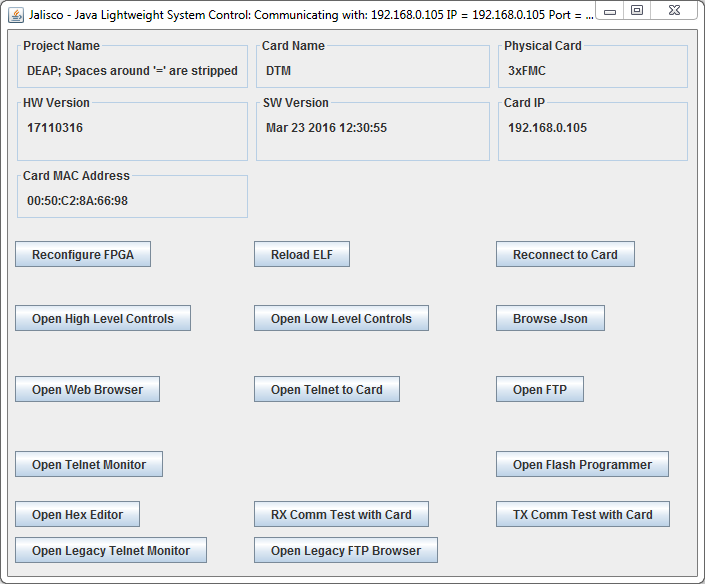
\includegraphics[width=.8\textwidth]{jaliscoTopScreen}
\caption{Main menu of \gls{jalisco} following startup.}
\label{Fig:jaliscoTopScreen}
\end{figure}

\clearpage

\section{Loading Firmware}
\NOTE{See the \href{https://edev.triumf.ca/projects/edevel00365/wiki/Boot_Sequence_and_Boot_Image_Selection}{EDEV page for more information.}}

\begin{figure}[ht]
\centering
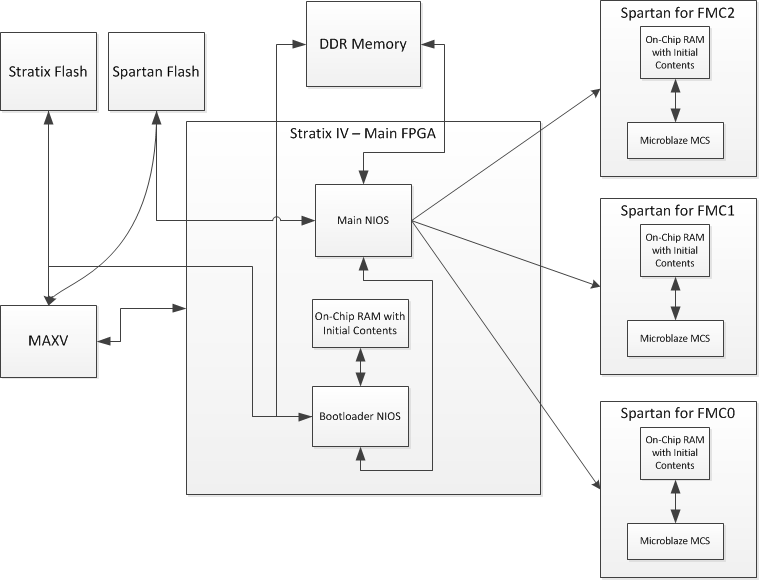
\includegraphics[width=\textwidth]{dtmDataStorage}
\caption{General layout of the FPGA, Embedded Processors, and Memory Devices on the \gls{dtm}. Photo Credit EDEV Department (\url{https://edev.triumf.ca/projects/edevel00365/wiki/Boot_Sequence_and_Boot_Image_Selection}).}
\label{Fig:dtmDataStorage}
\end{figure}

The installation of new firmware is done one of three different ways\footnote{To date (July 2016) only JTAG loading is used}: JTAG, FTP/Telnet, $\&$ via \gls{jalisco}. The safest method to update the firmware is over FTP. % FIXME (procedure outlined in Section \ref{sec:ftpLoading}). 
There are two versions of each flash image loaded as outlined in the following section (\ref{sec:dualImages}). Once the various FPGA images are loaded into the respective flash locations, the power is cycled loading the new firmware. 

\NOTE{Once a new image has been loaded check the \gls{jalisco} timestamp (see Section \ref{sec:jalisco})}

\subsection{Dual Load Images}
\label{sec:dualImages}
There are two images loaded onto the flash normally. The general concept is that there is a “normal image” or what should be used in normal operation and the image that is updated using \gls{jalisco} or FTP, and a “fallback image” that, for safety, cannot be modified via \gls{jalisco} nor FTP (only via JTAG) so it is far less susceptible to corruption. If an issue is detected with the primary image the secondary one will be used. 

There are three parts to a complete image load and it is crucial that the correct pairing of files is done.
\begin{enumerate}
\item Hardware (.pof) image of the Stratix FPGA
\item Software Image for the Main Nios (.elf)
\item Software and Hardware images for Spartans on FMC 0, FMC1, and FMC2 (.hex)
\end{enumerate}

Compiling of a new firmware release should be requested from the primary developer (Yair Linn\footnote{yairlinn@triumf.ca}).
The address map of the Stratix and the Spartan Flash images are shown in Fig. \ref{Fig:stratixImageFile} and \ref{Fig:spartanImageFile}.%\FIXME{WHAT IS THE TOP ADDRESS OF THESE?}.

\definecolor{lightgray}{gray}{0.8}
\begin{figure}
	\begin{bytefield}{12}
		\begin{rightwordgroup}{Stratix IV Dual Image}
			\memsection{0x0}{0x1000000}{3}{Page 0 - Normal Hardware Image (.pof)}\\
			\memsection{}{0x2000000}{3}{Normal Software Image (.elf)}\\
			\memsection{}{0x3000000}{3}{Page 1 - Fallback Hardware Image (.pof)}\\
			\memsection{}{0x3FFFFFF}{3}{Fallback Software Image (.elf)}
		\end{rightwordgroup}\\
	\end{bytefield}
	\caption{The address map of a Stratix IV flash file.}
	\label{Fig:stratixImageFile}
\end{figure}

\begin{figure}
	\begin{bytefield}{24}
		\begin{rightwordgroup}{Spartan-6 Dual Images}
			\memsection{0x0}{0x200000}{3}{FMC0 Normal Image}\\
			\memsection{}{0x400000}{3}{FMC1 Normal Image}\\
			\memsection{}{0x600000}{3}{FMC2 Normal Image}\\
			\memsection{}{0x800000}{3}{FMC0 Fallback Image}\\
			\memsection{}{0xA00000}{3}{FMC1 Fallback Image}\\
			\memsection{}{0xBFFFFF}{3}{FMC2 Fallback Image}\\
		\end{rightwordgroup} \\
		\memsectioncolor{0xC00000}{0x3FFFFFF}{6}{lightgray}{Unused}
	\end{bytefield}
	\caption{The address map of the flash file for the three \gls{fmc} boards}
	\label{Fig:spartanImageFile}
\end{figure}




On bootup the \gls{dtm} will pull these images from the flash and make a decision on which to use\footnote{For more on the startup sequence before this step see \url{https://edev.triumf.ca/projects/edevel00365/wiki/Boot_Sequence_and_Boot_Image_Selection\#Advanced-behind-the-scenes-view-of-boot-sequence}}

\subsubsection{Updating and Verifying Images}
\begin{description}
\item[EDEV Page: ]\hypNote{Link}{https://edev.triumf.ca/projects/edevel00365/wiki/Boot_Sequence_and_Boot_Image_Selection\#Updating-and-Verifying-the-images}{Link}
\end{description}

In order to avoid accidental overwriting of the fallback image, the only way to modify the fallback image is with a complete programming of the flashes via JTAG via the do\_program\_stratix\_flash.cmd and do\_program\_spartan\_flash.cmd commands. These commands each program their entire respective images as shown in Fig. \ref{Fig:stratixImageFile} $\&$ \ref{Fig:spartanImageFile}. Both the normal and fallback images are reflashed. It is intended that reprogramming via JTAG should be used infrequently, leaving the fallback image the same with the normal images being updated via \gls{jalisco} or FTP.


%\FIXME{Image verification, how is the normal/fallback image selected? just using these?}
On bootup the loaded images are checked and verified, if the normal images are found to have issues then the fallback images are used instead to ensure bootability.

\subsubsection{Choosing Flash Images}
\begin{description}
\item[EDEV Page: ]\href{ https://edev.triumf.ca/projects/edevel00365/wiki/Boot_Sequence_and_Boot_Image_Selection\#Choosing-Which-Image-Will-be-UsedChoosing-which-image-will-be-used-is-done-by-running-a-script-from-the-Nios-Command-Shell-from-the-tsbipscripts-directory-as-usual-To-select-the-normal-image-run-the-following-script}{Link}\footnote{\url{https://edev.triumf.ca/projects/edevel00365/wiki/Boot_Sequence_and_Boot_Image_Selection}}
\end{description}

Choosing which of the two images will be used is done by running a script from the Nios Command Shell (located in tsb/ip/scripts).

\begin{description}
\item [Load the normal image:] source do\_switch\_to\_normal\_flash\_image.cmd
\item [Load fallback image:] source do\_switch\_to\_fallback\_flash\_image.cmd
\end{description}

These scripts program the MaxV on-chip User Flash Memory via the JTAG with the correct settings to select the appropriate image. The script needs to be run only once; bootups after will default to this selected image until the other script is run to select the other image. These scripts take about 10 seconds to run, resulting in fast, easy switching between images.


%\subsection{JTAG}
%\label{sec:jtagProgramming}
%\begin{description}
%\item[JTAG Boot Sequence Monitoring:  ]\hypNote{Link}{https://edev.triumf.ca/projects/edevel00365/wiki/Boot_Sequence_and_Boot_Image_Selection\#Monitoring-the-boot-sequence}
%\end{description}


%\subsection{VME Hosting and Readout}

%\subsection{FTP}
%\label{sec:FTP}
%
%\subsubsection{FTP $\&$ Telnet Loading}
%\label{sec:ftpLoading}
%
%\FIXME{WHAT IS TELNET???}
%
%\begin{description}
%\item[EDEV Page:  ]\hypNote{Stratix Loading}{https://edev.triumf.ca/projects/edevel00365/wiki/Writing_of_Stratix_Flash_via_FTP_and_Telnet}, \hypNote{Spartan Loading}{https://edev.triumf.ca/projects/edevel00365/wiki/Writing_of_Spartan_Flash_via_FTP_and_Telnet}
%\end{description}
%FTP $\&$ Telnet loading is the preferred image loading method, the binary files are loaded onto the SD card on the SFP and Mini-SAS \gls{fmc} via FTP and then programmed to the appropriate FPGA flash using telnet. This loading method is, of course only available using edevel00365 as the top project.
%
%The Flash file needs to be a binary file that is generated and present in every release since t\_a\_release\_024 in the tsb/ip/exe directory. 
%\begin{description}
%\item[Stratix IV Binary:] stratix\_sof\_and\_elf\_image\_cropped.rbf
%\item[FMC0 Binary:] fmc0\_download\_raw\_bin.bin
%\item[FMC1 Binary:] fmc1\_download\_raw\_bin.bin
%\item[FMC2 Binary:] fmc2\_download\_raw\_bin.bin
%\end{description}
%This file needs to be transferred via FTP (which is run using \gls{jalisco}, see Section \ref{sec:jalisco}). This can be done using \gls{jalisco}'s FTP tool or any standard FTP tool. The user/password combination is triumf and triumf. Transfer mode must be binary (not ASCII).
%
%To run using \gls{jalisco}, once connected to the board, select 'open FTP' on the home screen (shown in Fig. \ref{Fig:jaliscoTopScreen}) which will open the FTP browser shown in Fig. \ref{Fig:ftpTopScreen}.\FIXME{THEN WHAT? HOW DO YOU CONNECT PROPERLY?}
%
%\begin{figure}[ht]
%\centering
%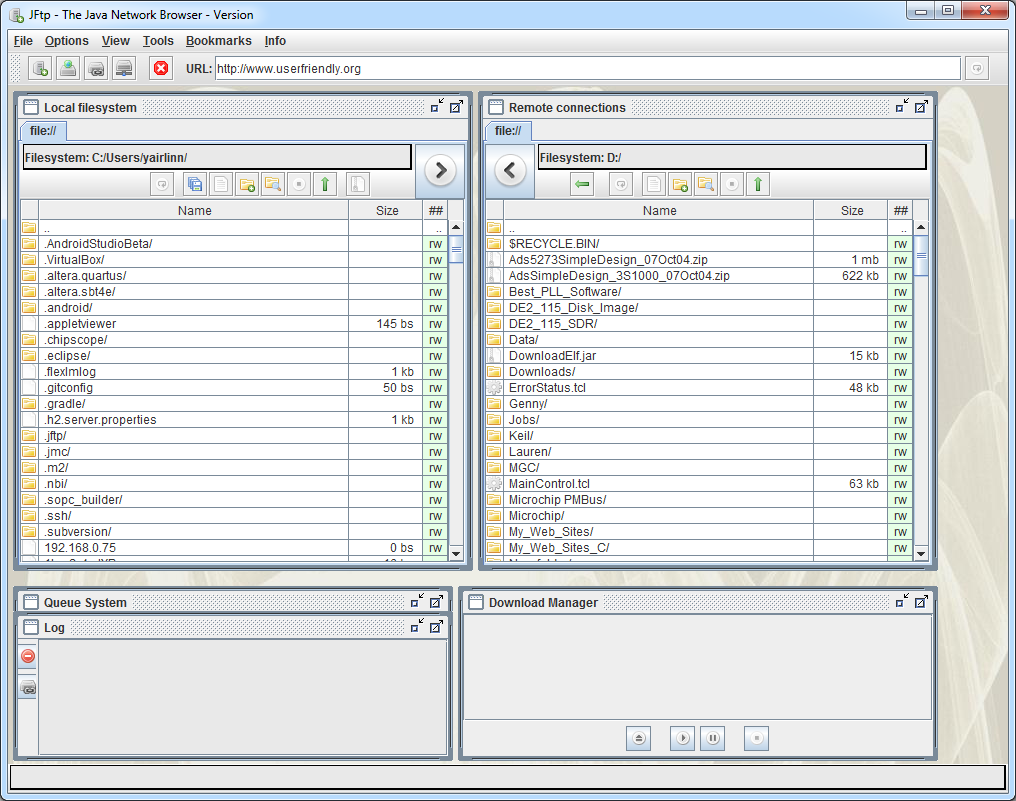
\includegraphics[width=\textwidth]{ftpTopScreen}
%\caption{General layout of the FPGA, Embedded Processors, and Memory Devices on the \gls{dtm}. Photo Credit EDEV Department (\url{https://edev.triumf.ca/projects/edevel00365/wiki/Boot_Sequence_and_Boot_Image_Selection}).}
%\label{Fig:ftpTopScreen}
%\end{figure}
%
%
%\textbf{Statix Programming}
%
%Connection to Telnet can be done via port 30 (manual command console, can be opened in Jalisco ("Open Telnet to Card") if desired) or, if desired (though not recommended) port 40 (for computer-based command interaction, which can be operated manually nonetheless). Connection should be in raw socket mode, standard telnet also seems to work well, but definitely do not use SSH.
%
%\begin{description}
%\item[Programming command:] program\_stratix\_hex\_file filename\footnote{filename is nominally stratix\_sof\_and\_elf\_image\_cropped.rbf}.
%\end{description}
%
%Programming of the flash in this method takes about 1 hour. This is due to Altera's Flash programming utilities which exhibit this performance. The time is basically limited by Altera's NIOS Flash programming board support package routines. It is unclear why those functions are four times slower than JTAG programming, and investigation is on-going as to whether this can be improved. Faster programming times will be seen if there are few changes to the binary image, in which case some unchanged blocks will not be rewritten.
%\FIXME{IS THIS STILL SLOW?}
%
%
%\textbf{Spartan Programming}
%
%Connection to Telnet can be done via port 30 (manual command console) or, if desired (though not recommended) port 40 (for computer-based command interaction, which can be operated manually nonetheless). Connection should be in raw socket mode, standard telnet also seems to work well, but definitely do not use SSH.
%
%\begin{description}
%\item[Programming command:] program\_spartan\_hex\_file filename fmc\_num
%\end{description}
%Here fmc\_num is the desired FMC so to program fmc0\_download\_raw\_bin.bin to FMC 0, the command is \textit{program\_spartan\_hex\_file fmc0\_download\_raw\_bin.bin 0}.
%
%This method allows for the programming of one \gls{fmc} at a time instead of all at once. Programming of a single FMC flash can take around 5 minutes, limited by Altera's NIOS Flash programming board support package routines. Faster programming times will be seen if there are few changes to the binary image, in which case some unchanged blocks will not be rewritten.
%
%\subsubsection{FTP Hosting}
%\subsubsection{FTP Readout}
%\begin{description}
%\item[EDEV Page:  ]\hypNote{proper readout}{https://edev.triumf.ca/projects/edevel00365/wiki/DMA_to_UDP_Transfers}
%\hypNote{manual or very low trigger rate operation}{https://edev.triumf.ca/projects/edevel00365/wiki/Software_DMA_Transactions}
%\end{description}
%
